%!TEX TS-program = xelatex
%!TEX encoding = UTF-8 Unicode
% !TEX root = ../../2017-GS-COME01-INVITO-ASCOLTO.tex

%-------------------------------------------------------------
%----------------------------- SUONO. SEGNO. INTERPRETAZIONE -
%-------------------------------------------------------------

\chapter*{Suono. Segno. Interpretazione.}
\addcontentsline{toc}{chapter}{Suono. Segno. Interpretazione.}

	\begin{flushright}
		\textit{Nella nostra anima c'\`e una incrinatura che, se sfiorata, \\
		risuona come un vaso prezioso riemerso dalle profondit\`a della terra} \\
		Wassilly Kandinsky - \emph{Lo Spirituale nell'Arte}
	\end{flushright}

	\begin{flushright}
		\textit{Music of Changes // John ChAnGEs} \\
		Pierre Boulez
	\end{flushright}

	\begin{flushright}
		\textit{Si dice che i compositori abbiano orecchio per la musica e \\
		di solito significa che non sentono nulla che arrivi alle loro orecchie. \\
		Le loro orecchie sono murate dai suoni di loro creazione.} \\
		John Cage - \emph{45' for a Speaker} (1954)
	\end{flushright}

\bigskip

%\begin{multicols}{2}

Le percezioni cambiano con il tempo. Ci sono diversi tempi, anche simultanei, del cambiamento.
Il tempo ciclico della riflessione. È quello breve, del pensiero ricorsivo, che non torna mai su se stesso identico al se stesso precedente.
In questo tempo la percezione stratifica, l'oggetto di senso percepito, osservato, muta, ne evolve il significato.
L'apparente movimento ciclico del pensiero ricorsivo non si muove ad anello, bensì in una sorta di spirale per cui sì, bidimensionalmente, può apparire un ritornare, ma ad una visione almeno tridimensionale questo appare a forma di spirale.
Quadrimensionalmente questa è una spirale che si muove nel tempo, che quindi occupa uno spazio temporale ampio, del divenire. Due tempi quindi, quello ciclico, ricorsivo, e quello lungo, della mutazione nelle spazio-tempo.

\begin{tikzpicture}[segment amplitude=10pt]
  \draw[snake=coil]                  (0,1) -- (3,1);
  %\draw[snake=coil,segment aspect=0] (0,0) -- (3,0);
\end{tikzpicture}

A queste percezioni che mutano nel tempo e nello spazio siamo abituati a dare nomi. Suono, è un nome.
L'idea di suono è separata dalla cosa che rappresenta.
Potremmo dire che il suo significato è rimasto quasi invariato nel corso dei tempi
In questo gli studi etimologici sono strumenti indispensabili.
Il rapporto sensoriale che identificheremo con le parole cambiano però piuttosto rapidamente.
Con la parola suono definiamo una percezione. Definiamo suono una percezione.
Il suo significato risale a epoche antiche.

Le arti del tempo condividono la stessa struttura percettiva: un testo fissato ed il suo alter ego evento momentaneo.

\begin{quote}
	la scrittura in tutti i campi si costituisce nel momento in cui si può disporre di un sistema di marcatori visivi che assolvono a fruizioni precedentemente affidate alla memoria o ad altri artifici più rudimentali\footnote{borio 9}
\end{quote}

Suono e Segno. I due stati dell'oggettivazione musicale sui quali l'interpretazione, sguardo ad oggettività limitata, vede collegamenti e potenzialità. Suono e gesto viaggiano su un asse temporale diverso da quello della sua rappresentazione. Ma circoscrivere il segno a “semplice” rappresentazione è grossolanamente sbagliato.

Se suono e gesto possiedono un tempo separato da quella della sua rappresentazione (tradizione orale) allora c'è da domandarsi cosa la scrittura abbia aggiunto e se si è verificata una eventuale perdita.

\begin{quote}
	il testo musicale [\ldots] solleva una pretesa normativa di fronte a chi lo legge\footnote{Borio}.
\end{quote}

Non ci vuole molto ad ipotizzare quindi una perdita di spontaneità e fantasia espressiva dell'interprete contemporaneo, incatenato alle regole scritte più del suo collega libero, che usava le parole piuttosto che i segni per imbrigliare il discorso musicale. Evidentemente quindi potrebbe risultare la perdita di spontanea immaginazione nel rapporto con il solo istinto musicale. Non si può nemmeno ignorare il fatto che è la forma scritta a regolare al tempo funzione informativa ed evolutiva tale da strutturare complesse relazioni orizzontali e verticali riconoscibili dalla memoria. Il segno che permette al raginamento di formare il tempo musicale. La scrittura come sistema di relazione tra segni nel tempo.

\begin{quote}
	la sua efficacia è strettamente connessa alla precisione e alla rapidità con cui vengono riconosciuti i simboli e i loro composti, cioè i tempi e modi con cui si svolge la lettura del testo\footnote{Borio}.
\end{quote}

L'evento momentaneo nella espressione della sua unicità è legato nel tempo stesso all'arte che rappresenta attraverso lo sguardo, la voce e il gesto dell'interprete. L'interpretazione nelle arti del tempo è manifestazione di una storia parallela a quella della percezione, della scrittura, e della pratica musicale. L'interpretazione è di fatto una riscrittura nel tempo del tempo. Ma ci deve essere una differenza tra l'interpretazione nel dominio orale piuttosto che scritto.

\begin{quote}
	lun discorso lineare e non ripetittivo per non parlare di una costruzione sillogistica, presuppine l'esistenza di un \emph{MEDIUM} che permetta alla psiche di sospendere le sue relazioni immediate; la scrittura è particolarmente adatta a tale scopo\footnote{Borio 14}.
\end{quote}

Nella composizione del percorso musicale quindi la pratica di scrittura è un mezzo per gestire limiti psico-cognitivi doiversi tra soggetti diversi. Non è quindi un paragone disumano tra oralità e scrittura quanto ognuno di questi in relazione all'uomo che li produce.

\begin{quote}
	alla base della scrittura moderna vi è dunque un processo di astrazione mediante cui il discorso temporale viene raffigurato nella successine spaziale\footnote{Borio 15}.
\end{quote}

Suono, evento momentaneo.

Segno, discorso temporale astratto.

Interpretazione, lettura multi-sensoriale del tempo. Solo l'interpretazione può riconoscere il progetto musicale celato nel testo e nella sua identità sonora.

\begin{center}
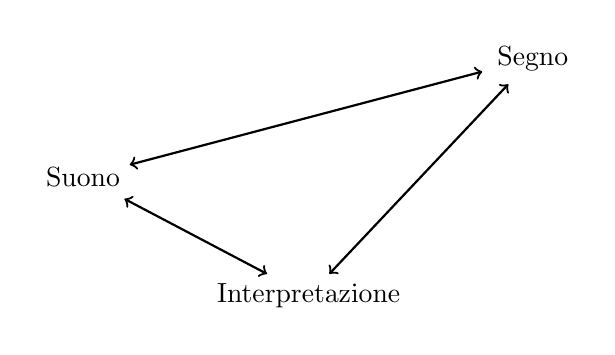
\begin{tikzpicture}[
    auto,
    arrow/.style = {
    	draw,
		thick,
		<->,
		shorten >=2pt
		}
  ]
\matrix [column sep=10mm, row sep=10mm] {
    & &	\node [] (segno) {Segno}; \\
	\node [] (suono) {Suono}; & &\\
    & \node [] (interpretazione) {Interpretazione}; &	 \\	
  };

\begin{scope} [every path/.style=arrow]
  	\path (suono) -- (segno);
	\path (interpretazione) -- (suono);
	\path (interpretazione) -- (segno);
\end{scope}
  
\end{tikzpicture}
\end{center}

\begin{quote}
	\ldots sono segni rivelatori delle cose, immagini delle parole, dotate di tal
	forza che, pur senza suono alcuno, ci trasmettono ciò che è stato detto da
	persone lontane: [le lettere, infatti, permettono alle parole di entrare in noi
	attraverso gli occhi e non attraverso l'udito]\footnote{controllare bene citazione isidoro di siviglia}
\end{quote}

questo vale quanto mai anche per la scrittura musicale, dove le “note” sono le immagini sonore dei suoni.


La musica, come le altre arti del tempo, danza, teatro, poesia presentano uno sdoppiamento su due piani dimensionali: testo ed evento.
La partitura musicale in particolare propone una dialettica tra testo e suoni che non si riscontra però in un copione o in notazioni coreografiche. Il testo stesso offre solo scansione metrica. Il testo musicale è prescrizione di un insieme di azioni e contemporaneamente è una prima oggettivazione di senso\footnote{Gianmario Borio, \emph{Segno e suono. Sulle funzioni della scrittura per la rappresentazione del pensiero musicale} in \emph{La scrittura come rappresentazione del pensiero musicale}. In nota Borio propone, per approfondimenti sull'esemplarità della notazione musicale nella relazione con una teoria generale dell'arte Nelson Goodman, \emph{I linguaggi dell'arte}}.

Queste considerazioni

%\end{multicols}

%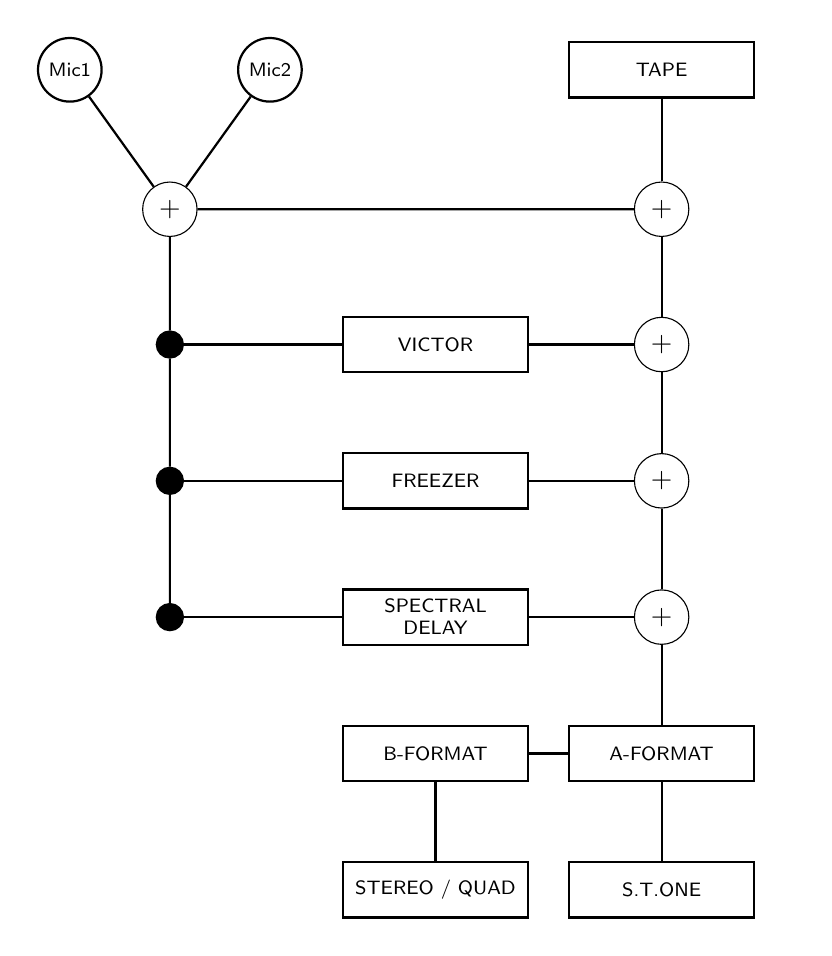
\begin{tikzpicture} [
    auto,
    mic/.style = {
    	font=\scriptsize\sffamily,
		circle,
		draw=black,
    	thick,
    	%fill=blue!20,
    	text width=2em,
    	text badly centered,
    	inner sep=1pt,
	},
    block/.style    = {
    	font=\scriptsize\sffamily,
    	rectangle,
		draw=black,
		thick,
		%fill=black!10,
		text width=6em,
		text centered,
		%rounded corners,
		minimum height=2em
		},
	line/.style = {
    	draw,
		thick,
		fill=black
		%shorten >=2pt
		},
	control/.style = {
    	draw,
		circle,
		thick,
		fill=black,
		%shorten >=2pt
		},
    arrow/.style = {
    	draw,
		thick,
		->,
		shorten >=2pt
		},
  ]
  % Define nodes in a matrix
  \matrix [column sep=5mm, row sep=10mm] {
	\node [mic] (mic1) {Mic1}; & \node [] (null1) {}; & \node [mic] (mic2) {Mic2}; & & \node [block] (tape) {TAPE}; & \\
	& \node [draw,circle] (inputs) {+}; & & & \node [draw,circle] (direct) {+}; & \\
	& \node [control] (node1) {}; & & \node [block] (victor) {VICTOR}; & \node [draw,circle] (mix1) {+}; & \\
	& \node [control] (node2) {}; & & \node [block] (freezer) {FREEZER}; & \node [draw,circle] (mix2) {+}; & \\
	& \node [control] (node3) {}; & & \node [block] (sdelay) {SPECTRAL DELAY}; & \node [draw,circle] (mix3) {+}; & \\
	& & & \node [block] (bfmt) {B-FORMAT}; & \node [block] (afmt) {A-FORMAT}; & \\
	& & & \node [block] (outputs) {STEREO / QUAD}; & \node [block] (stone) {S.T.ONE}; & \\
  };

  \begin{scope} [every path/.style=line]
  	\path (mic1) -- (inputs) -- (node1) -- (node2) -- (node3);
	\path (mic2) -- (inputs) -- (direct);
    \path (node1) -- (victor) -- (mix1);
    \path (node2) -- (freezer) -- (mix2);
    \path (node3) -- (sdelay) -- (mix3);
    \path (tape) -- (direct) -- (mix1) -- (mix2) -- (mix3);
    \path (mix3) -- (afmt) -- (stone);
    \path (afmt) -- (bfmt) -- (outputs);

  \end{scope}

\end{tikzpicture}

